\chapter{DataFlow Engine}

\section{Introduction}

In this chapter, a dataflow engine is presented based on the work detailed in \textit{An Extensible Virtual Machine Design for the Execution of High-Level Languages on Tagged-Token Dataflow Machines} \cite{saey_extensible_2017}.
	
This engine is designed to support parallel execution of instructions by queuing all operands to instructions and executing these in a scope agnostic way.
Tagged token dataflow is an extension to the data flow model where tags are used to distinguish the execution context of tokens, i.e. multiple invocations of the same instruction with different execution contexts, for example calling the same function twice (See section \ref{sec:tagged-token-dataflow}).
For the purposes of this thesis, a lightweight version of this engine has been implemented in Racket to facilitate the mapping process from FrDataFlow. Furthermore, we implemented a mapping layer that translates reactive signals to data flow instructions. Even though there were some mismatches that needed to be addressed, reactive programs can now be expressed in FrDataFlow and evaluated atop the dataflow engine. 

\newpage
\section{Architecture}

\subsection{Components}

The dataflow engine consists of three core components:

\begin{description}[style=nextline]
	\item[The token queue] This contains the tokens that need to be processed. A token has a value and meta data about which instruction it needs to be sent to. 
	\item[The matching memory] This stores the operands per instruction and per context. As long as not all inputs are present and the instruction is not ready to be invoked, these partial sets of inputs are kept here.
	\item[The execution unit] This unit will actually invoke the instructions with its operands
\end{description}

The interaction between these components can be seen in figure \ref{fig:engine-architecture-tokenprocessing}. 
What the dataflow engine essentially does is continuously pull tokens from the queue, send it through the matching memory which calls the execution unit. This will invoke the instruction with its operands, wrap the result in a token and put it on the queue again. 

\begin{figure}[h!]
	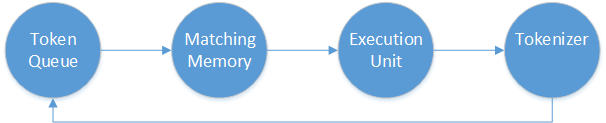
\includegraphics[width=\textwidth]{images/Engine-Architecture-TokenProcessing.png}
	\caption{The interaction between the three components of the dataflow engine}
	\label{fig:engine-architecture-tokenprocessing}
\end{figure}

\newpage

For clarity, figure \ref{fig:background-dataflow-token-again} is repeated here (from the Background chapter) to reiterate the structure of a token. 

\begin{figure}[ht]
	\centerline{\includegraphics[width=\textwidth]{images/background-dataflow-token.png}}
	\caption{A tagged token}
	\label{fig:background-dataflow-token-again}
\end{figure}


\subsection{Example program with evaluation by the dataflow engine}

Take for example a non reactive sample program which computes the average of two numbers, as shown in listing \ref{lst:engine-architecture-sample}

\begin{lstlisting}[caption={Computing the average of two numbers},captionpos=b,label={lst:engine-architecture-sample},language=FrDataFlow]
(define (average x y)
  (/ (+ x y) 2))
  
(average 2 6)
(average 1 5)
\end{lstlisting}

This program computes the average of two numbers twice using different arguments. When this program gets evaluated in the data flow engine, the four arguments and the 2s from the division by two are added to the token queue, containing information about which execution context they belong to and what should happen with the result. 
In this example, the 2 and 6 belong to the same execution context, while 1 and 5 will belong to a different one. 

\begin{figure}[h!]
	\centering
	\includegraphics[scale=0.8]{images/Engine-Architecture-1.png}
	\caption{The corresponding data flow nodes for two calls to the \textit{average} function. Each color represents a different execution context.}
	\label{fig:engine-architecture-1}
\end{figure}

In figure \ref{fig:engine-architecture-1} we see the arguments queued up against the \textit{plus} instruction. Colors indicate the execution context. At this point, the token queue consists of 2, 6, 1, 5 and two 2s. These values are all wrapped in a token containing meta data, i.e. the tag. 

\begin{figure}[h!]
	\centering
	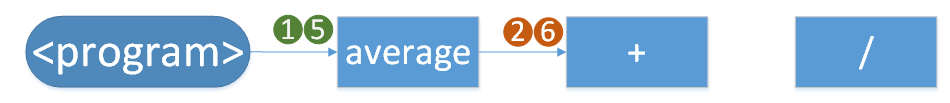
\includegraphics[scale=0.8]{images/Engine-Architecture-2.png}
	\caption{The results of the \textit{plus} instruction are forwarded to the \textit{divide} instruction}
	\label{fig:engine-architecture-2}
\end{figure}

Since all inputs are present for the first invocation, the \textit{plus} instruction gets invoked, as shown in figure \ref{fig:engine-architecture-2}. This adds a new token to the queue: 8. This result will serve as the input of the \textit{divide} instruction. 
The next thing that happens in figure \ref{fig:engine-architecture-3} is the same step for 1 and 5.

\begin{figure}[h!]
	\centering
	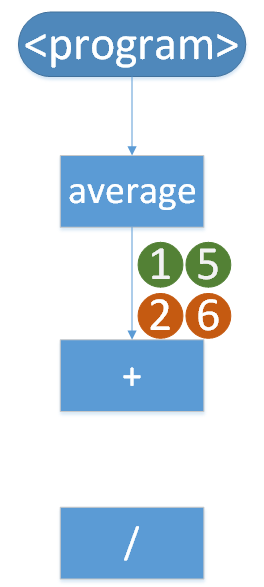
\includegraphics[scale=0.8]{images/Engine-Architecture-3.png}
	\caption{The second invocation of the \textit{plus} instruction finishes. All inputs are now present for the \textit{divide} instruction for both execution contexts.}
	\label{fig:engine-architecture-3}
\end{figure}

\begin{figure}[h!]
	\centering
	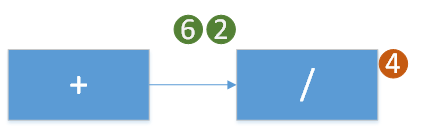
\includegraphics[scale=0.8]{images/Engine-Architecture-4.png}
	\caption{The first \textit{divide} instruction is invoked. Its result is put on the token queue again.}
	\label{fig:engine-architecture-4}
\end{figure} 

\begin{figure}[h!]
	\centering
	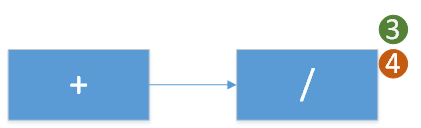
\includegraphics[scale=0.8]{images/Engine-Architecture-5.png}
	\caption{The second \textit{divide} instruction is invoked. Its result is put on the token queue again.}
	\label{fig:engine-architecture-5}
\end{figure}

Note that the tags are very important here, otherwise the engine would not be aware which inputs belong to the same invocation. There is no guarantee that tokens will always be enqueued in the correct order.

In the end, when the \textit{divide} instruction has also completed, its results are pushed into the token queue again, as shown by figure \ref{fig:engine-architecture-4} and \ref{fig:engine-architecture-5}. This allows further processing of the data, but is outside the scope of this example. 

To summarize, the dataflow engine processes tokens in the queue, invokes instructions whenever all of its inputs in one execution context are present and re-enqueues the results of those invocations. Separate function calls are distinguished using tags that denote the execution context.

\section{Mapping of reactive signals to dataflow engine}

To execute our reactive signals on the dataflow engine, a translation step was required to simulate the update loop using the described mechanisms in the dataflow engine.
When we represent reactive programming as a graph, the nodes are signals while the vertices denote dependencies between them.
In the dataflow model, the nodes are instructions and the vertices are data being passed in to them. Therefore, our mapping layers creates data flow nodes for every signal, where the arguments passed in are the parent signal values. When a new value is produced, a token is generated for every child that is subscribed to it.

Taking our example from the Language chapter, we have the following reactive program in figure \ref{fig:engine-mapping-1}.

\begin{figure}[h!]
	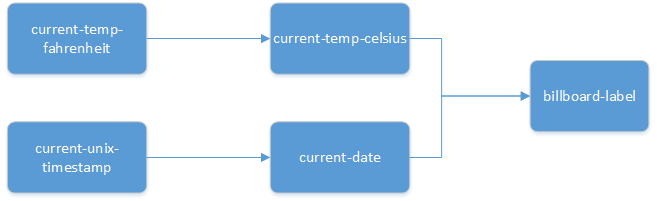
\includegraphics[width=\textwidth]{images/Engine-Mapping-1.png}
	\caption{The billboard program, but the signals are now data flow nodes}
	\label{fig:engine-mapping-1}
\end{figure}

This program behaves exactly the same as the reactive version, the only difference being that it is now running atop a dataflow engine.

\subsection{Updating signals on a dataflow runtime}

In reactive programs, signals with a dependency to two or more parent signals are updated whenever at least one of their parents emits a new value. This boils down to the signal functioning as a mapping of the latest values of its parents. Taking our example, this means that when the current temperature changes, the billboard will update immediately, even if the current date has not changed at all.
Similarly, the billboard label updates when the date changes, even if the temperature has not emitted a new value. In a sense, signals remember the latest values from each parent and reuse them whenever a new value from one of the parent comes in.

In the dataflow engine, an instruction that gets invoked consumes its tokens. Once the instruction has been invoked, the tokens are thrown away. This is problematic, because when the current temperature emits a new value, it produces a new token. The dataflow engine will assign this token to the billboard label node, but will keep waiting until the current date produces another token as well before invoking the billboard label again. This means that a signal which is now mapped as a dataflow node does not update until ALL of its parents have emitted new values. This is the biggest mismatch between the reactive model and the data flow model.

Simulating the behavior of reactive signals in the data flow model requires a way to retrieve the latest values of other parent signals when a new token arrives. 
Although each signal has references to all of its parents, it is not advisable to just read out the latest values and generate extra tokens for the other parents as well. This is because a strict requirement of the dataflow model is that nodes must be processed in isolation and cannot access shared state, which is what retrieving the latest values of the parents would amount to.  
This would break the potential for parallelism, because it should be presumed that these dataflow nodes live in and are invoked on separate processes and even machines. The whole premise of the dataflow model is that nodes are only allowed to access the incoming data from the tokens and nothing else.

We propose to simulate new signal emissions for all of the \textit{source signals} whenever one of them emits a new value. These are signals without parents that get updated by the runtime outside of the update loop. Since there is no language support for filtering, throttling or dynamically manipulating the flow of data through the graph, it can be safely assumed that emitting new values from the source signals will ripple through the entire graph, causing all nodes to be updated. In practice, this means that whenever a new temperature is sent out, the current seconds also pushes a value out at the same time. The necessary tokens for all of the source signals are put on the queue at the same time, simulating the required behavior: whenever one parent emits, the other parents do too. This results in the desired behavior: whenever one parent signal emits, the other parents do too so that all the children are recomputed, without having to memorize any of their parents' values. 

\newpage
\section{Conclusion}

In this chapter, we presented a tagged token dataflow engine. This is a runtime that enqueues arguments to instructions and executes these in parallel. 
When interpreting code in the FrDataFlow language, the reactive signals are mapped to dataflow nodes in the engine using a custom mapping layer. During this process, mismatches between reactive programming and the dataflow model are tackled. This is done by making all source signals emit new values whenever one of them has a new value, to avoid signals waiting in the dataflow engine for inputs from all their parents. Secondly, since return values are not supported in the dataflow engine, the decision was made to only model signals as dataflow instructions and leave the rest of the code execution inside the original interpreter code. 
In the end, we have a reactive system running atop a parallel dataflow engine, triggering updates in the correct way whenever a parent signal emits. 





